\RequirePackage{paralist}
\documentclass[full,kernel]{l3doc}
\usepackage[dvipsnames]{xcolor}
\usepackage[utf8]{inputenc}
\usepackage[T1]{fontenc}
\RequirePackage{morewrites}
\RequirePackage{tikzinput}
\usetikzlibrary{fit}

\usepackage[debug=all,lang=en, mathhub=./tests]{stex}
\usepackage{url,array,float,textcomp}
\usepackage[show]{ed}
\usepackage[hyperref=auto,style=alphabetic]{biblatex}
\addbibresource{\bibfolder/kwarcpubs.bib}
\addbibresource{\bibfolder/extpubs.bib}
\addbibresource{\bibfolder/kwarccrossrefs.bib}
\addbibresource{\bibfolder/extcrossrefs.bib}
\usepackage{amssymb}
\usepackage{amsfonts}
\usepackage{xspace}
\usepackage{hyperref}

\makeindex
\floatstyle{boxed}
\newfloat{exfig}{thp}{lop}
\floatname{exfig}{Example}

\usepackage{listings}
\usepackage{lststex}

\lstdefinelanguage{sTeX}{
  sensitive=true,
  numbers=left,
  numbersep=3pt,
  xleftmargin=3pt,
  alsodigit={\$},
  %gobble=4,
  alsoletter={\\},
  %moredelim = [s][\itshape]{$}{$},
  %moredelim = [s][\itshape\bfseries]{\\[}{\\]},
  classoffset=0,keywordstyle=\bfseries,morekeywords={
      \\begin,\\end,\\ExplSyntaxOn,\\ExplSyntaxOff,\\documentclass,
      \\usepackage,\\def,\\[,\\],\\else,\\fi,$\iffalse$\fi,
      \\newcommand, \\renewcommand, \\let
  },	
  classoffset=1,keywordstyle=\itshape\color{OliveGreen},morekeywords={
      \\defeq,\\geometricSeries,\\infinitesum,\\realdivide,
      \\realpower,
      \\symbolname,\\binarysymbol,\\newbinarysymbol,\\addition,
      \\summation,\\ascendingchain,\\quantforall,\\set,\\funtype,
      \\Nat,\\successor,\\multiplication,\\Int,\\zero,\\uminus,
      \\intmonoid
  },	
  classoffset=2,keywordstyle=\color{blue},morekeywords={
    \\symdecl,\\symdef,\\notation,\\vardef,\\varseq,\\instantiate,
    \\varinstantiate, \\renamedecl, \\assign, \\setnotation,
    \\STEXexport
  },
  classoffset=3,keywordstyle=\color{BurntOrange},morekeywords={
    \\importmodule,\\usemodule,\\libinput,\\inputref,\\mhinput,
    \\libusepackage,\\addmhbibresource,\\ifinputref
  },
  classoffset=4,keywordstyle=\color{Purple},morekeywords={
    \\definiendum,\\definame,\\symref,\\symname,\\comp,
    \\compemph,\\definiens,\\svar,\\infprec,\\neginfprec,\\ellipses,
    \\Symname,\\arg
  },
  classoffset=5,keywordstyle=\color{magenta},morekeywords={
    smodule,sdefinition,sassertion,sparagraph,sproof,
    copymodule,interpretmodule,mathstructure,sexample
  }
}

%\lstdefinestyle{mylatex}{	
%	keywordstyle=\color{BurntOrange}
%}
%\lstdefinelanguage{mylatex}{
%	emphstyle=\underbar,
%	alsodigit={:},
%	%alsoletter={_},
%	alsoletter={\\}
%	sensitive=true,
%	classoffset=0,keywordstyle=\bfseries,
%	morekeywords={\\begin,\\end,\\ExplSyntaxOn,\\ExplSyntaxOff},	
%	classoffset=1,keywordstyle=\color{blue},
%	morekeywords={
%		\\symdecl,
%		\\symdef,
%		\\notation,
%		\\abbrdef,
%		\\importmodule,
%		\\usemodule,
%		\\STEXwithbrackets,
%		\\symref
%	},
%	classoffset=2,keywordstyle=\color{Purple},
%	morekeywords={
%		\\stex_path_from_string:Nn,
%		\\stex_path_to_string:NN,
%		\\stex_path_to_string:N,
%		\\stex_require_repository:n,
%		\\stex_modules_current_namespace:,
%		\\stex_debug:n,
%		\\stex_set_current_repository:n,
%		\\stex_file_in_smsmode:nn,
%		\\stex_get_symbol:n,
%	},
%	classoffset=3,keywordstyle=\color{SkyBlue},
%	morekeywords={
%		\\l_stex_modules_ns_str,
%		\\g_stex_currentfile_seq,
%		\\l_stex_current_module_prop,
%		\\l_stex_get_symbol_uri_str,
%	}
%	classoffset=0,
%%^^A	morecomment=[l][\color{Gray}]{//},
%%^^A	morecomment=[s][\color{Gray}]{/*}{*/},
%	morecomment=[s][\color{Green}]{$}{$},,
%	morecomment=[s][\color{OliveGreen}]{\\[}{\\]},
%^^A  morestring=[b][\color{Purple}]\$,
%}
\lstnewenvironment{latexcode}[1][]{\lstset{language=sTeX,#1}}{}

\def\stexcode{\lstinline[language=sTeX]}

\usepackage{mdframed,realboxes}
\usepackage[most]{tcolorbox}
\usepackage{caption}

\newenvironment{framed}{\begin{mdframed}\begin{center}}{\end{center}\end{mdframed}}
\newcommand{\scaled}[2][0.9\hsize]{\begin{center}\resizebox{#1}{!}{\begin{minipage}{\textwidth} #2 \end{minipage}}\end{center}}

\newenvironment{stextest@output}
{
  \begin{mdframed}[linewidth=1pt,backgroundcolor=white]\small
}
{\end{mdframed}}

\newenvironment{stextest@input}
{
  \begin{mdframed}[linewidth=1pt,backgroundcolor=white]\small
}
{\end{mdframed}}

\makeatletter

\newcount\test@counter\test@counter=0
\newcount\example@counter\example@counter=0

\newtcolorbox{exampleborderbox}{
  empty,
  title={Example \the\example@counter},
  attach boxed title to top left,
     minipage boxed title,
  boxed title style={empty,size=minimal,toprule=0pt,top=1pt,left=3mm,overlay={}},
  coltitle=blue,fonttitle=\bfseries,
  parbox=false,boxsep=0pt,left=3mm,right=0mm,top=2pt,breakable,pad at break=0mm,
     before upper=\csname @totalleftmargin\endcsname0pt, 
  overlay unbroken={\draw[blue,line width=2pt] ([xshift=-0pt]title.north west) -- ([xshift=-0pt]frame.south west); },
  overlay first={\draw[blue,line width=2pt] ([xshift=-0pt]title.north west) -- ([xshift=-0pt]frame.south west); },
  overlay middle={\draw[blue,line width=2pt] ([xshift=-0pt]frame.north west) -- ([xshift=-0pt]frame.south west); },
  overlay last={\draw[blue,line width=2pt] ([xshift=-0pt]frame.north west) -- ([xshift=-0pt]frame.south west); },
  outer arc=4pt
}


%\newtcolorbox{exampleborderbox}{
%  enhanced,
%  left=0pt,
%  title={Example \the\example@counter},
%  right=0pt,
%  top=8pt,
%  bottom=8pt,
%  colback=white,
%  colframe=blue,
%  width=\textwidth,
%  enlarge left by=0mm,
%  boxsep=5pt,
%  fontupper=\small,
%  arc=4pt,
%  outer arc=4pt,
%  leftupper=1.5cm,
%  fonttitle=\bfseries,
%  coltitle=blue,
%  boxed title style={empty,size=minimal,toprule=0pt,top=1pt,left=3mm,overlay={}},
%}

\newenvironment{example@border}
{
  \global\advance\example@counter by 1
%^^A\refstepcounter{remark}
\begin{exampleborderbox}
}
{\end{exampleborderbox}}

 \makeatother
 
\def\present#1{\texttt{>>\meaning#1<<}}
\def\printltx#1{\texttt{\detokenize{#1}}}

\newwrite\testoutfile
\def\testfile{0}

\ExplSyntaxOn

\def\stexexample{
  \begingroup 
  \catcode`\\=12\relax
  \catcode`\#=12\relax
  \catcode`\&=12\relax
  \catcode`\$=12\relax
  \catcode`\^=12\relax
  \catcode`\_=12\relax
  \catcode`\ =12\relax
  \catcode`^^J=12\relax
  \endlinechar=`^^J
  \newlinechar=-1
%^^A    \everyeof{\noexpand}
  \example_a:n
}
\long\def\example_a:n #1 {
  \endgroup
  \begin{example@border}
    \immediate\openout\testoutfile=stextest.tst
    \immediate\write\testoutfile{
      \c_backslash_str begin{latexcode}
      \detokenize{^^J}#1
      \c_backslash_str end{latexcode}
    }
    \immediate\closeout\testoutfile

    Input:

    \begin{stextest@input}
      \catcode`\#=12\relax
      \input{stextest.tst}
    \end{stextest@input}
    \immediate\openout\testoutfile=stextest.tst
    \immediate\write\testoutfile{#1}
    \immediate\closeout\testoutfile

    Output:
    
    \begin{stextest@output}
      \input{stextest.tst}
    \end{stextest@output}
  \end{example@border}
}

\ExplSyntaxOff

\newtcolorbox{dangerbox}{
  breakable,
  enhanced,
  left=0pt,
  right=0pt,
  top=8pt,
  bottom=8pt,
  colback=white,
  colframe=red,
  width=\textwidth,
  enlarge left by=0mm,
  boxsep=5pt,
  fontupper=\small,
  arc=4pt,
  outer arc=4pt,
  leftupper=1.5cm,
  overlay={
    \node[anchor=west] at ([xshift=10pt]$(frame.north west)!0.5!(frame.south west)$)
       {
\includegraphics[width=1cm,height=1cm]{stex-dangerous-bend}};}
}

\usetikzlibrary{decorations.pathmorphing,shapes,arrows,calc}
% Taken from pgflibrarytikzmmt.code.tex
\newcommand{\mmtarrowtip}{angle 45}
\newcommand{\mmtarrowtipmonoright}{right hook}

\tikzstyle{include}=[\mmtarrowtipmonoright-\mmtarrowtip,thick]
\tikzstyle{morph}=[-\mmtarrowtip,thick]
\tikzstyle{preview}=[decorate, decoration={coil,aspect=0,amplitude=1pt,
                                                  segment length=6pt,
                                                  pre=lineto,pre length=3pt,
                                                  post=lineto,post length=5pt}, thick]
\tikzstyle{view}=[preview,-\mmtarrowtip]

% TIKZ RULES
\def\mmtlogo{
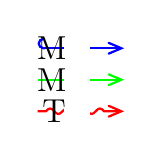
\begin{tikzpicture}

  % White Background (Margins are eyeballed)
  % This is necessary because we paste white over arrows later.
  % If somebody want's to do the full song and dance with
  % interrupted arrows to get transparent background, be my guest.

  \fill[white!] (-0.01,0.15) rectangle (1.11,-0.95);

  % Arrows
  \draw [blue, include] (0,0)     -- (1.1,0);
  \draw [green, morph] (0,-0.4)  -- (1.1,-0.4);
  \draw [red, view]   (-0,-0.8) -- (1.1,-0.8);

  % Cutout for letters
  \fill[white] (0.33,0.1) rectangle (0.66,-0.9);

  % Letters
  \node at (0.18,0)    (nodeM1) {\large M};
  \node at (0.18,-0.4) (nodeM2) {\large M};
  \node at (0.21,-0.8) (nodeT)  {\large T};

\end{tikzpicture}
}

\newtcolorbox{mmtbox}{
  breakable,
  enhanced,
  left=0pt,
  right=0pt,
  top=8pt,
  bottom=8pt,
  colback=white,
  colframe=green,
  width=\textwidth,
  enlarge left by=0mm,
  boxsep=5pt,
  fontupper=\small,
  arc=4pt,
  outer arc=4pt,
  leftupper=1.5cm,
  overlay={
    \node[anchor=west] at ([xshift=10pt]$(frame.north west)!0.5!(frame.south west)$)
       {\mmtlogo};}
}


\MakeShortVerb{\|}

\def\scsys#1{{{\sc #1}}\index{#1@{\sc #1}}\xspace}
\def\mmt{\textsc{Mmt}\xspace}
\def\xml{\scsys{Xml}}
\def\mathml{\scsys{MathML}}
\def\omdoc{\scsys{OMDoc}}
\def\openmath{\scsys{OpenMath}}
\def\latexml{\scsys{LaTeXML}}
\def\perl{\scsys{Perl}}
\def\cmathml{Content-{\sc MathML}\index{Content {\sc MathML}}\index{MathML@{\sc MathML}!content}}
\def\activemath{\scsys{ActiveMath}}
\def\twin#1#2{\index{#1!#2}\index{#2!#1}}
\def\twintoo#1#2{{#1 #2}\twin{#1}{#2}}
\def\atwin#1#2#3{\index{#1!#2!#3}\index{#3!#2 (#1)}}
\def\atwintoo#1#2#3{{#1 #2 #3}\atwin{#1}{#2}{#3}}
\def\cT{\mathcal{T}}\def\cD{\mathcal{D}}

\def\fileversion{3.0}
\def\filedate{\today}

\RequirePackage{pdfcomment}

\ExplSyntaxOn\makeatletter
\cs_set_protected:Npn \@comp #1 #2 {
  \pdftooltip {
    \textcolor{blue}{#1}
  } { #2 }
}

\cs_set_protected:Npn \@defemph #1 #2 {
  \pdftooltip { 
    \textbf{\textcolor{magenta}{#1}}
  } { #2 }
}

\def\__omtext_lec#1{#1}
\cs_new_protected:Npn \lec #1 {
  \strut\hfil\strut\null\hfill\__omtext_lec{#1}
}
\makeatother\ExplSyntaxOff

\makeatletter
\let\@stex@oldcomment\comment
\let\@stex@oldendcomment\endcomment

%\RequirePackage{comment}
\RequirePackage{document-structure}
\RequirePackage[hints,solutions,notes]{problem}
\RequirePackage{hwexam}

\let\comment\@stex@oldcomment
\let\endcomment\@stex@oldendcomment

\newif\ifinfulldoc\infulldocfalse
\makeatother

\def\basedocurl{https://github.com/slatex/sTeX/blob/latex3/doc}
\newcounter{module}

\NewDocumentEnvironment {module}{}{
  \stepcounter{module}
  \textbf{Module \themodule: \smoduletitle}
}{

}
\stexpatchmodule[visible]{\begin{module}}{\end{module}}

\usepackage{stexthm}


\newtcolorbox{remarkbox}[1][]{
  empty,
  title={Remark \theremark: #1},
  attach boxed title to top left,
      minipage boxed title,
  boxed title style={empty,size=minimal,toprule=0pt,top=4pt,left=3mm,overlay={}},
  fonttitle=\bfseries,coltitle=black,
  before=\par\medskip\noindent,parbox=false,boxsep=0pt,left=3mm,right=0mm,top=2pt,breakable,pad at break=0mm,
      before upper=\csname @totalleftmargin\endcsname0pt, 
  overlay unbroken={\draw[black,line width=2pt] ([xshift=-0pt]title.north west) -- ([xshift=-0pt]frame.south west); },
  overlay first={\draw[black,line width=2pt] ([xshift=-0pt]title.north west) -- ([xshift=-0pt]frame.south west); },
  overlay middle={\draw[black,line width=2pt] ([xshift=-0pt]frame.north west) -- ([xshift=-0pt]frame.south west); },
  overlay last={\draw[black,line width=2pt] ([xshift=-0pt]frame.north west) -- ([xshift=-0pt]frame.south west); },
}

\renewenvironment{remark}[1][]{
  \refstepcounter{remark}\begin{remarkbox}[#1]
  \begin{mdframed}[linewidth=1pt,backgroundcolor=lightgray!33!white]
}{
\end{mdframed}\end{remarkbox}\endlist
}